\documentclass{article}
\usepackage[utf8]{inputenc}
\usepackage[a4paper, margin=1in]{geometry}
\usepackage{graphicx}

\title{Visualizing the Decline in Cultural Participation in Europe Post-Crisis}
%\author{Omar Lizardo}
\date{March 2023}

\begin{document}

\maketitle

\begin{abstract}
    Previous work in cultural sociology shows that trends in cultural participation, if they exist, tend to be slow and gradual, responding to cohort changes and impervious to period-specific events. Here I use data from the two Eurobarometer surveys fielded just before (2007) and in the immediate aftermath (2013) of the great recession related eurozone crisis to visualize the impact of a once in a generation period-specific shock for the four national cases most deeply affected: Portugal, Spain, Italy, and Greece. In all cases, with the possible exception of Spain, can observe steep increases in rates of non-participation affecting particularly the less-educated, except for Greece, for which we can see general negative impacts of the crisis on participation across all levels of education. \end{abstract}

\section{Introduction}
Previous work shows that while trends in cultural participation across societies are rarely completely static, any changes we observe usually follow the timescale of cohort replacement, namely, gradual and relatively slow. Thus, while in some cases we observe systematic trends upwards or downwards as tastes for specific activities change across generations (DiMaggio, 2004), we are more likely to observe continuity and ``inertia'' seemingly impervious to period-specific factors like changes in cultural policy or trends in the globalization of cultural production (Coulangeon, 2013; López-Sintas \& Katz-Gerro 2005).

A twin set of Eurobarometer surveys containing a cultural participation module allows us to revisit the idea of the preponderance of inertia and gradual change in cultural participation trends. The surveys were fielded in 2007 and 2013. They thus provide us with an opportunity to estimate the impact of a major exogenous, period-specific shock of generational significance: Namely, the global financial crisis and its aftermath the ``Great Recession,'' the most severe global recession since the great depression in the early 20th century,  affecting all the world's rich economies most significantly. In Europe, in particular, the great recession led to the {\em eurozone debt crisis}, which brought the economies and financial systems of various Southern European economies (including the cases analyzed here) to their knees, visiting extreme economic hardship on the populace.

In what follows, I visualize the impact of the financial crisis on cultural participation using data on the immediate ``before''---Eurobarometer 67.1, fielded in Februrary-March 2007---and ``after''---Eurobarometer 79.2, fielded in April-May 2013---(European Commission, 2012; 2016). The two data sets contain matching cultural participation items across six activities: (1) Going to the movies, (2) Attending a dance performance, (3) Attending a museum or a gallery, (4) Attending a musical concert, (5) Visiting a historical monument, and (6) attending a dramatic or theater performance. I focus my analysis on the four Southern European economies most deeply affected by the crisis: Portugal, Spain, Italy, and Greece. The analysis is limited to respondents aged twenty or older who report having completed schooling. 

\section{The decline in cultural participation post-crisis}
Figure~\ref{fig: main} shows stacked bar plots designed for the analysis and presentation of Likert-type data (Heiberger \& Robins 2014), rendered using the {\em} {\em R} package \texttt{likert} developed by Bryer \& Speerschneider (2016).\footnote{The color palette used in the plot is ``Royal2" from Karthik Ram's (2018) \texttt{wesanderson} {\em R} package.}  Looking at the top-left panel, depicting data from all survey respondents, we can see that three of the four Southern European countries---except Spain---experienced noticeable increases in cultural non-participation post-crisis. This is indicated in each panel in the figure by a leftward shift of the bottom stacked bar (built from 2017 responses) relative to the top bar (built from 2007 responses). As the plot shows, the proportion of people reporting no cultural activities goes from 54\%, 47\%, 35\%, and 28\% in 2007 for Portugal, Greece, Spain, and Italy, to 64\%, 58\%, 38\%, and 37\%, respectively. 

Is there heterogeneity in the decline in cultural participation across respondents with different levels of education? We know from previous work that education is the best predictor of cultural participation and that the cultural participation habits of the more educated are more resistant to exogenous shocks. Moreover, education is correlated with earnings, which means that any restrictions on leisure consumption for cultural goods should hit the less educated the hardest. Looking at the top-right and bottom panels of the plot, we find that the decline in cultural participation affected people with more and less education differently in each national case. However, across all four national cases, we can observe noticeable increases in the proportion of people with less education abstaining from cultural participation in 2013 compared to 2007.  We can see that the decline in cultural participation post-crisis is steepest among respondents who report completing their education between the ages of sixteen and nineteen (roughly a high-school or vocational education). In Portugal, the percentage of abstainers in this category almost doubles, going from 24\% in 2007 to 41\% in 2013, and an increase of similar substantive magnitude can be observed in Greece (36\% versus 56\%), with less dramatic but still substantial increases in non-participation among this category of respondents in Spain (19\% versus 26\%) and Italy (15\% versus 27\%). This is a substantial negative shock in the cultural practices of people with less cultural capital, seldom observed in previous studies of arts participation.

What about the cultural participation behavior of the more educated? In Portugal, Spain, and Italy, respondents who report completing their education at the age of twenty or older, corresponding roughly to some university education or a more advanced degree, do not experience substantively significant increases in abstention across periods. The exception is university-educated Greeks, who went from 15\% abstainers in 2007, a number comparable to the other Southern European cases, to 26\% in 2013, the highest among all Southern European national cases within the university-educated ranks and closer to the rates of abstainers among \textit{high-school educated} respondents in Spain and Italy. In 2013, University-educated Greeks were also the least well-represented in the avid (five to six activities) participation category across all four national cases compared to people of similar educational attainment, suggesting that the Eurozone crisis had a significant impact on the cultural participation behavior of even the most cultural-capital privileged members of the Greek population. By way of contrast, the avid-participation category actually \textit{grew} among university-educated Portuguese, going from 22\% pre-crisis to 31\% post-crisis.

Thus, there appears to be a connection between the intensity with which the financial and debt crises hit a particular country and subsequent state and civil-society responses to the crisis---as Greece was the most deeply affected of the Southern European economies---and the extent to which the effects of the crisis were restricted to those with less cultural and economic resources or impacted the entirety of the population. 

\begin{figure}
    \centering
    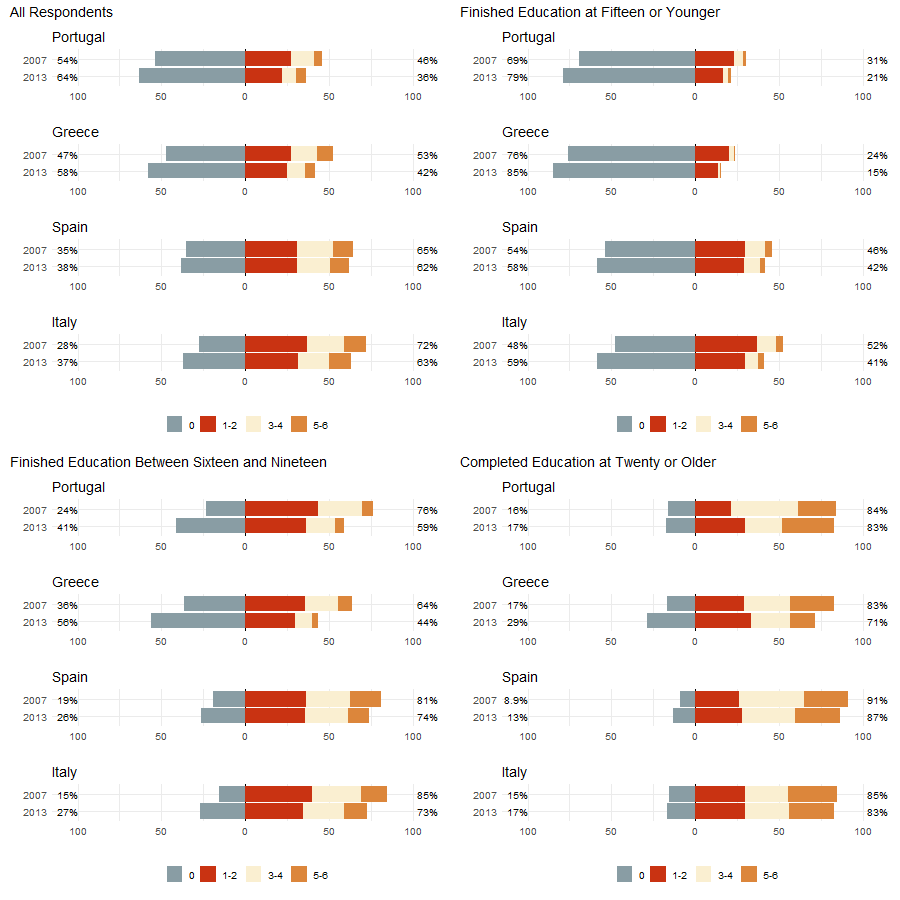
\includegraphics[width=1.0\textwidth]{Plots/cult-cat-by-year-by-country-combo.png}
    \caption{Stacked bar plots of the number of cultural activities reported by individuals in the previous year for four Southern European countries calculated from Eurobarometer survey data from 2007 (pre-Eurozone crisis) and 2013 (post-crisis). Each horizontal bar represents four ordered categories of participation: None, one to two, three to four, and five to six cultural activities, with each response category represented by different colored bar segments. Horizontal bars are centered at the zero category (vertical line intersecting the x-axis at zero) such that the percentages listed at the left of the gray bar represent the proportion of nonparticipating respondents, and the percentages listed at the right of each bar represent the proportion of respondents who participated in at least one cultural activity. As evident in the leftward within-country shift of the bottom horizontal bar---corresponding to 2013 responses---compared to the top bar, we can observe a substantively significant increase in non-participation across all four national cases, with the steepest declines observed among individuals who completed their education between the ages of sixteen and nineteen (bottom-right panel), and minimal shifts in the participation behavior of the university educated, except for Greece.}
    \label{fig: main}
\end{figure}

\section*{References}
\noindent

Bryer, J., \& Speerschneider, K. (2016). Package ‘likert’. Likert: Analysis and Visualization Likert Items, version 1.3, 5, 2016.

Coulangeon, P. (2013). Changing policies, challenging theories and persisting inequalities: Social disparities in cultural participation in France from 1981 to 2008. \textit{Poetics}, 41(2), 177-209.

DiMaggio, P., \& Mukhtar, T. (2004). Arts participation as cultural capital in the United States, 1982–2002: Signs of decline? \textit{Poetics}, 32(2), 169-194.

European Commission (2012). Eurobarometer 67.1 (Feb-Mar 2007). GESIS Data Archive, Cologne. ZA4529 Data file Version 3.0.1. 

European Commission (2016). Eurobarometer 79.2 (Apr-May 2013). GESIS Data Archive, Cologne. ZA5688 Data file Version 6.0.0, 

Heiberger, R., \& Robbins, N. (2014). Design of diverging stacked bar charts for Likert scales and other applications. Journal of Statistical Software, 57, 1-32.

López-Sintas, J., \& Katz-Gerro, T. (2005). From exclusive to inclusive elitists and further: Twenty years of omnivorousness and cultural diversity in arts participation in the USA. \textit{Poetics}, 33(5-6), 299-319.

Ram, K. (2018). wesanderson: a Wes Anderson palette generator. R package version 0.3, 6, 2018.

\end{document}
